
\begin{example}{interconnection of hybrid systems $\HS_1$ (bouncing ball) and $\HS_2$ (moving platform)}
\label{ex:interconnection1}
Consider a bouncing ball ($\HS_1$) bouncing on a platform ($\HS_2$) at some initial height and converging to the ground at zero height. This is an interconnection problem because the current states of each system affect the behavior of the other system. In this interconnection, the bouncing ball will contact the platform, bounce back up, and cause a jump in height of the platform so that it gets closer to the ground. After some time, both the ball and the platform will converge to the ground. In order to model this system, the output of the bouncing ball becomes the input of the moving platform, and vice versa. For the simulation of the described system with regular data where $\HS_1$ is given by

\begin{eqnarray}
f_1(\xi, u_1,v_1):=\left[
 \begin{array}{c}
   \xi_2 \\
 -\gamma - b\xi_2 +v_{11}
 \end{array}
\right],
   C_1 : = \defset{(\xi,u_1)}{\xi_1 \geq u_1, u_1 \geq 0}\\
g_1(\xi, u_1, v_1):=\left[ \begin{array}{c}
 \xi_1+\alpha_1\xi_2^2 \\
e_1|\xi_2| + v_{12}
\end{array}
\right]\ ,
    D_1: =\defset{(\xi,u_1)}{\xi_1 =u_1, u_1 \geq 0},
y_1 = h_1(\xi) : =\xi_1
\end{eqnarray}
where $\gamma, b, \alpha_1 >0, e_1 \in [0,1)$, $\xi = [\xi_1 , \xi_2]^\top$ is the state, $y_1 \in \Re$ is the output, $u_1 \in \Re$ and $v_1 = [v_{11} , v_{12}]^\top \in \Re^{2}$ are the inputs, and the hybrid system $\HS_2$ is given by

\begin{eqnarray}
f_2(\eta,u_2,v_2):=\left[
 \begin{array}{c}
   \eta_2 \\
 -\eta_1-2\eta_2 +v_{12}
 \end{array}
\right],
   C_2 : = \defset{(\eta,u_2)}{\eta_1 \leq u_2, \eta_1 \geq 0}\\
g_2(\eta,u_2,v_2):=\left[ \begin{array}{c}
 \eta_1-\alpha_2|\eta_2| \\
-e_2|\eta_2| + v_{22}
\end{array}
\right]\ ,
    D_2: =\defset{(\eta,u_2)}{\eta_1 = u_2, \eta_1 \geq 0},
y_2 = h_2(\eta) : = \eta_1
\end{eqnarray}
where $\alpha_2 >0, e_2 \in [0,1)$, $\eta = [\eta_1 , \eta_2]^\top \in \Re^{2}$ is the state,
$y_2 \in \Re$ is the output, and $u_2 \in \Re$ and $v_2 = [v_{21} , v_{22}]^\top \in \Re^{2}$
are the inputs.

Therefore, the interconnection may be defined by the input assignment
\begin{equation}
u_1 = y_2,   \hspace{5mm}     u_2 = y_1.
\end{equation}

The signals $v_1$  and $v_2$ are included as external inputs in the model in order to simulate the effects of environmental perturbations, such as a wind gust, on the system.

The MATLAB scripts in each of the function blocks of the implementation above are given as follows. The constants for
the interconnected system are $\gamma = 0.8$, $b=0.1$, and $\alpha_1, \alpha_2=0.1$.

\begin{figure}[ht!]
  \begin{center}
    {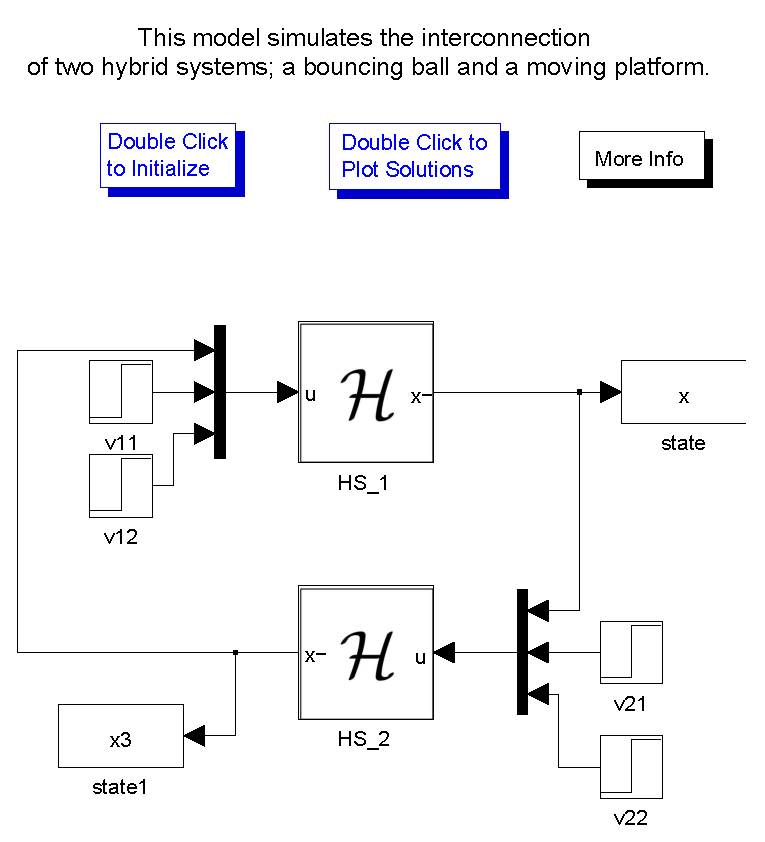
\includegraphics[width=.6\textwidth]{figures/Simulink/InterconnectionMdl.eps}}
   \caption{MATLAB/Simulink implementation of interconnected hybrid systems $\HS_1$ and
$\HS_2$}
\label{fig:interconnection-1}
  \end{center}
\end{figure}

\begin{figure}[ht!]
  \begin{center}
  \psfrag{flows [t]}[c]{flows [$t$]}
  \psfrag{jumps [j]}[c]{jumps [$j$]}
  \psfrag{xi1, eta1}[c]{$\xi_1, \eta_1$}
  \psfrag{xi2, eta2}[c]{$\xi_2, \eta_2$}
    {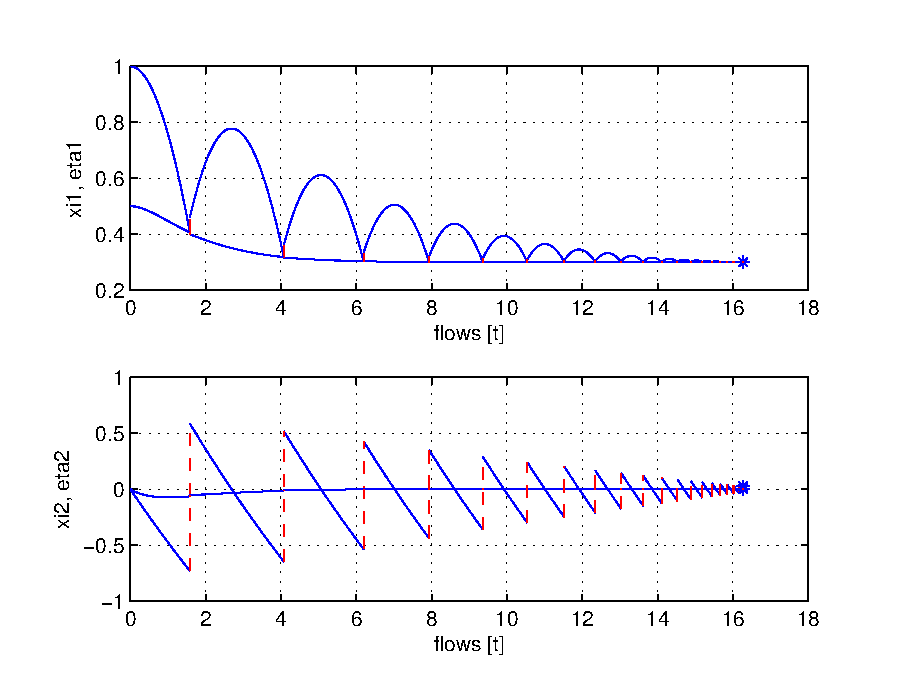
\includegraphics[width=.8\textwidth]{figures/Examples/InterconnectionH1H2.eps}}
   \caption{Solution of Example~\ref{ex:interconnection1}: height and velocity}
\label{fig:interconnection-2}
  \end{center}
\end{figure}

%\begin{figure}[ht]
%  \begin{center}
%  \psfrag{flows [t]}[c]{flows [$t$]}
%  \psfrag{jumps [j]}[c]{jumps [$j$]}
%  \psfrag{xi1}[c]{$\xi_1$}
%    {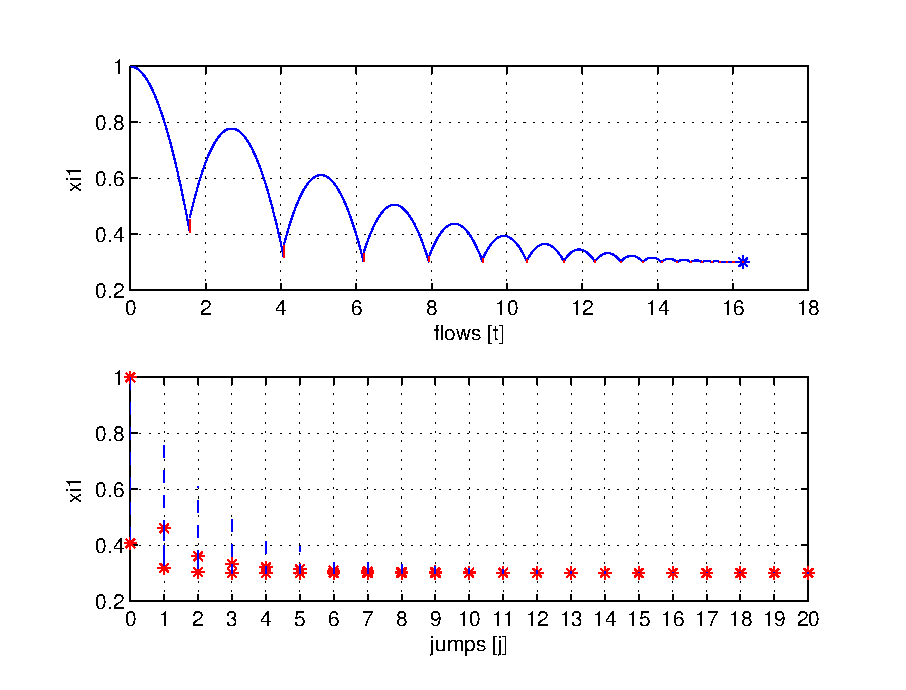
\includegraphics[width=.8\textwidth]{figures/Examples/InterconnectionH1.eps}}
%   \caption{Solution of Example~\ref{ex:interconnection1} for system $\HS_1$: height}
%\label{fig:interconnection-3}
%  \end{center}
%\end{figure}
%
%\begin{figure}[ht]
%  \begin{center}
%  \psfrag{flows [t]}[c]{flows [$t$]}
%  \psfrag{jumps [j]}[c]{jumps [$j$]}
%  \psfrag{xi2}[c]{$\xi_2$}
%    {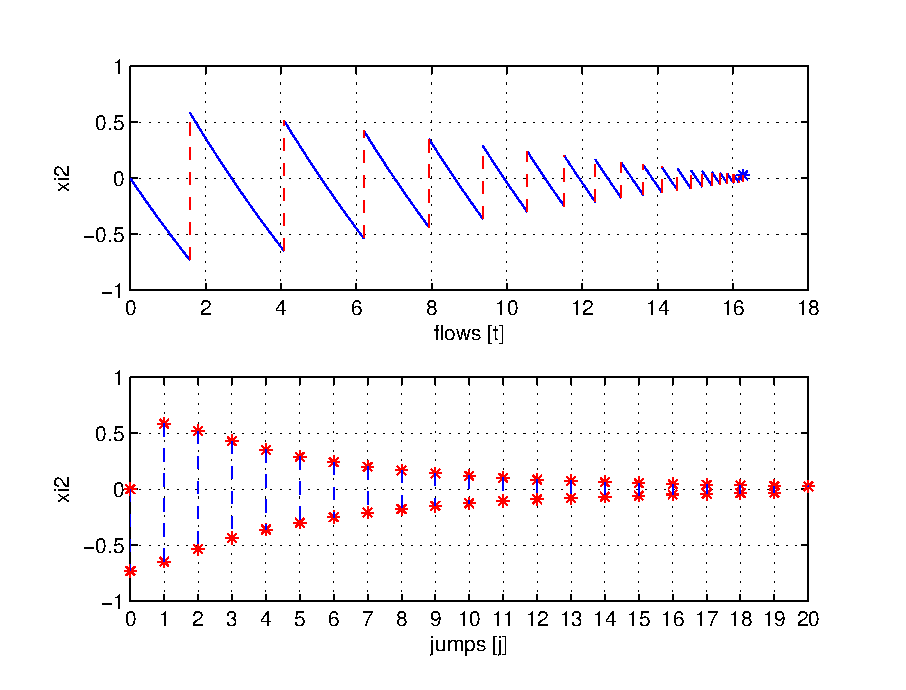
\includegraphics[width=.8\textwidth]{figures/Examples/InterconnectionH1velocity.eps}}
%   \caption{Solution of Example~\ref{ex:interconnection1} for system $\HS_1$: velocity}
%\label{fig:interconnection-4}
%  \end{center}
%\end{figure}

\begin{figure}[ht]
  \centering
  \psfrag{flows [t]}[c]{flows [$t$]}
  \psfrag{jumps [j]}[c]{jumps [$j$]}
  \psfrag{xi1}[c]{$\xi_1$}
  \psfrag{xi2}[c]{$\xi_2$}
\subfigure[Height]{
    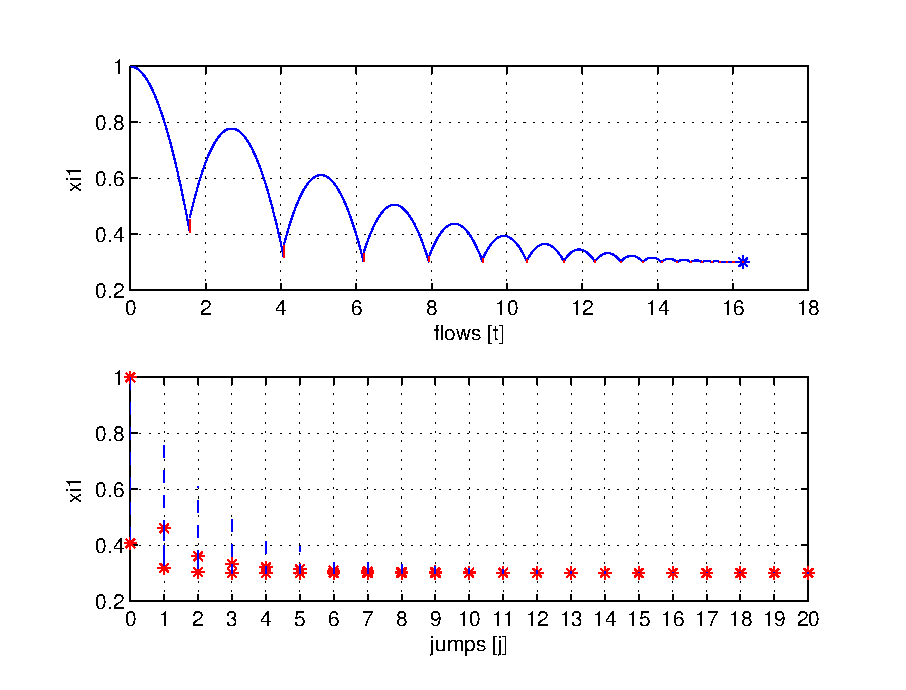
\includegraphics[width=.45\textwidth]{figures/Examples/InterconnectionH1.eps}
\label{fig:interconnection-3}}
\qquad
\subfigure[Velocity]{
    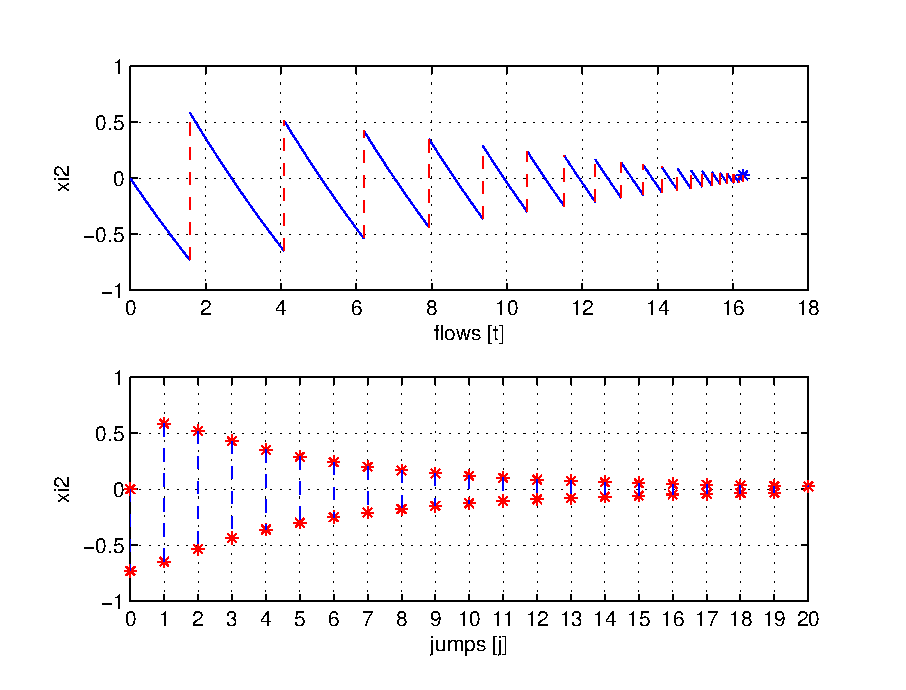
\includegraphics[width=.45\textwidth]{figures/Examples/InterconnectionH1velocity.eps}
\label{fig:interconnection-4}}
\caption{Solution of Example \ref{ex:interconnection1} for system $\HS_1$}
\end{figure}

%\begin{figure}[ht]
%  \begin{center}
%  \psfrag{flows [t]}[c]{flows [$t$]}
%  \psfrag{jumps [j]}[c]{jumps [$j$]}
%  \psfrag{eta1}[c]{$\eta_1$}
%    {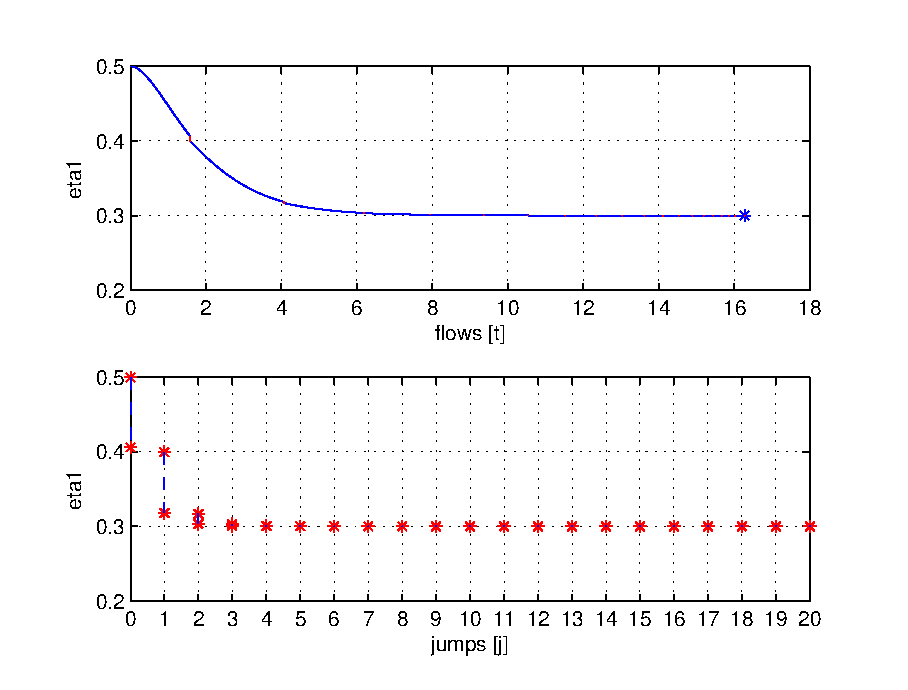
\includegraphics[width=.8\textwidth]{figures/Examples/InterconnectionH2.eps}}
%   \caption{Solution of Example~\ref{ex:interconnection1} for system $\HS_2$: height}
%\label{fig:interconnection-5}
%  \end{center}
%\end{figure}
%
%\begin{figure}[ht]
%  \begin{center}
%  \psfrag{flows [t]}[c]{flows [$t$]}
%  \psfrag{jumps [j]}[c]{jumps [$j$]}
%  \psfrag{eta2}[c]{$\eta_2$}
%    {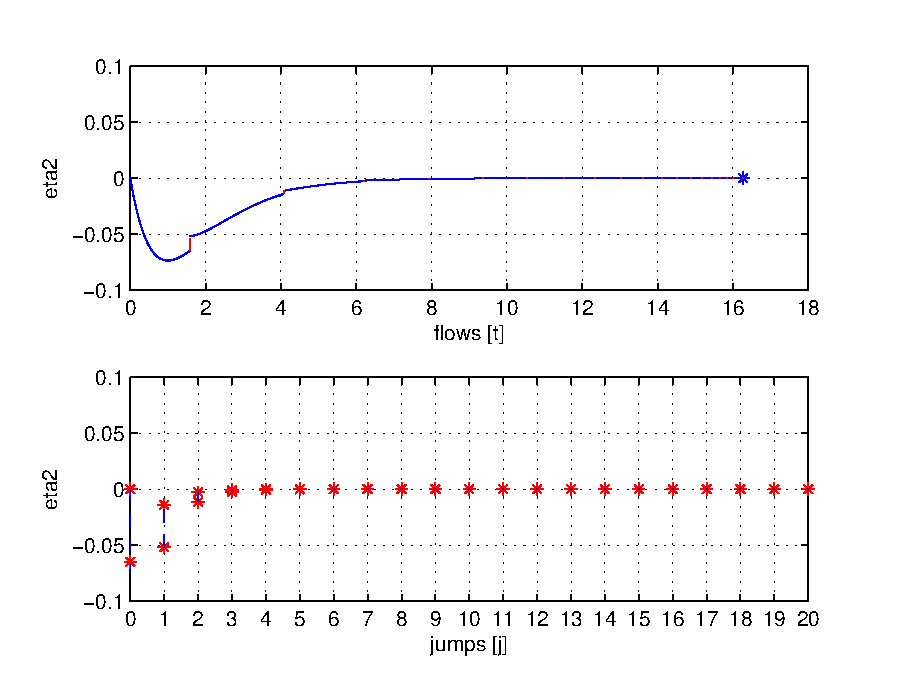
\includegraphics[width=.8\textwidth]{figures/Examples/InterconnectionH2velocity.eps}}
%   \caption{Solution of Example~\ref{ex:interconnection1} for system $\HS_2$: velocity}
%\label{fig:interconnection-6}
%  \end{center}
%\end{figure}

\begin{figure}[ht]
  \centering
  \psfrag{flows [t]}[c]{flows [$t$]}
  \psfrag{jumps [j]}[c]{jumps [$j$]}
  \psfrag{eta1}[c]{$\eta_1$}
  \psfrag{eta2}[c]{$\eta_2$}
\subfigure[Height]{
    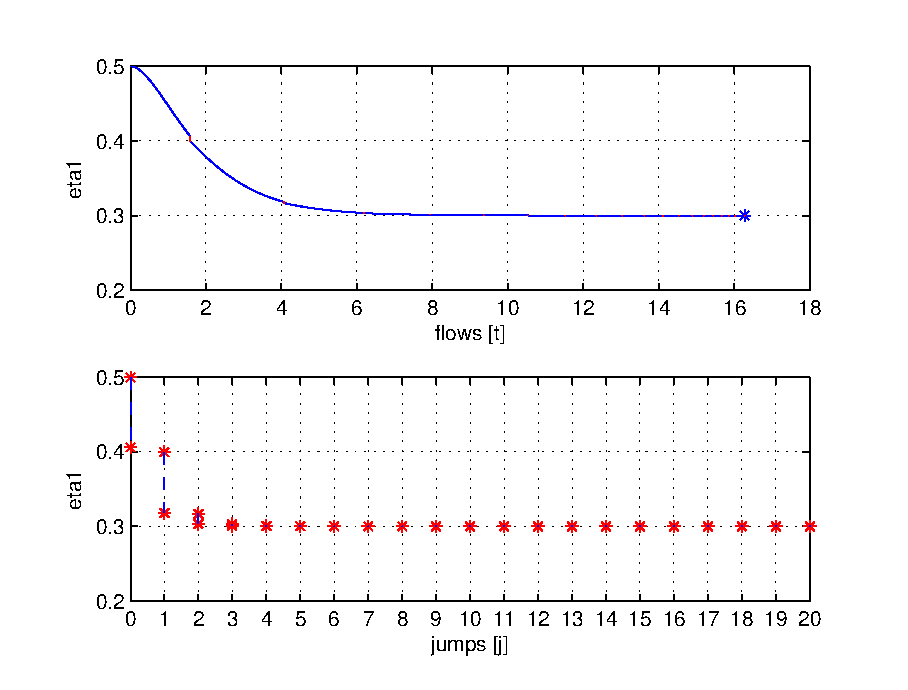
\includegraphics[width=.45\textwidth]{figures/Examples/InterconnectionH2.eps}
\label{fig:interconnection-5}}
\qquad
\subfigure[Velocity]{
    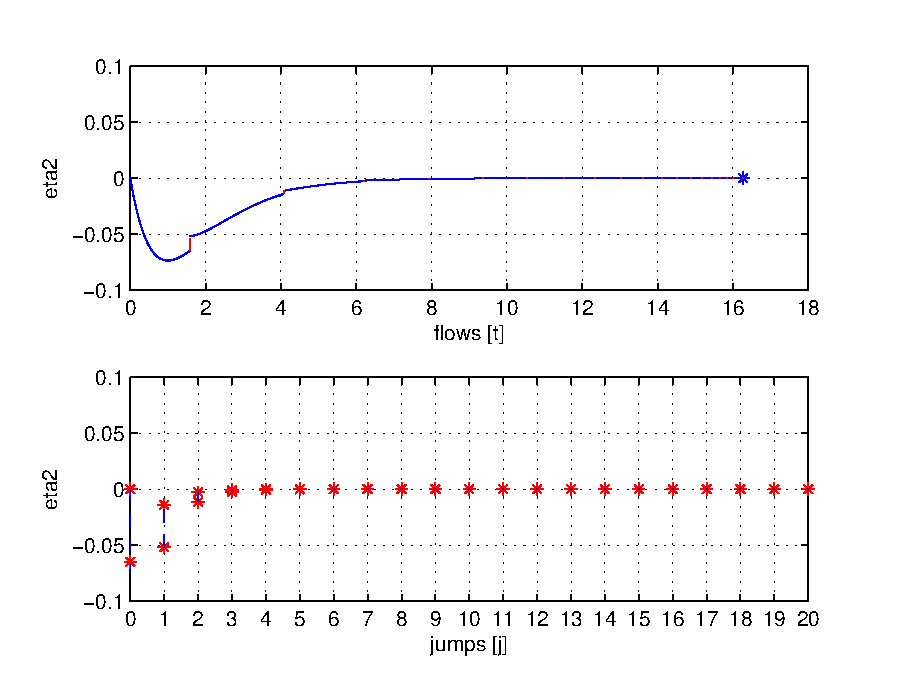
\includegraphics[width=.45\textwidth]{figures/Examples/InterconnectionH2velocity.eps}
\label{fig:interconnection-6}}
\caption{Solution of Example~\ref{ex:interconnection1} for system $\HS_2$}
\end{figure}

% Set the location for MATLAB files included via the "\code" command.
\codeLocation{Matlab2tex_1_6}

\begin{itemize}
\item For hybrid system $\HS_1$:

\code{f.m}
\code{C.m}
\code{g.m}
\code{D.m}

% Flow map
% %\scriptsize
% % This file was automatically created from the m-file 
% "m2tex.m" written by USL. 
% The fontencoding in this file is UTF-8. 
%  
% You will need to include the following two packages in 
% your LaTeX-Main-File. 
%  
% \usepackage{color} 
% \usepackage{fancyvrb} 
%  
% It is advised to use the following option for Inputenc 
% \usepackage[utf8]{inputenc} 
%  
  
% definition of matlab colors: 
\definecolor{mblue}{rgb}{0,0,1} 
\definecolor{mgreen}{rgb}{0.13333,0.5451,0.13333} 
\definecolor{mred}{rgb}{0.62745,0.12549,0.94118} 
\definecolor{mgrey}{rgb}{0.5,0.5,0.5} 
\definecolor{mdarkgrey}{rgb}{0.25,0.25,0.25} 
  
\DefineShortVerb[fontfamily=courier,fontseries=m]{\$} 
\DefineShortVerb[fontfamily=courier,fontseries=b]{\#} 
  
\noindent                    
 \hspace*{-1.6em}{\scriptsize 1}$  $\color{mblue}$function$\color{black}$ xdot = f(x, u, gamma)$\\
 \hspace*{-1.6em}{\scriptsize 2}$  $\\
 \hspace*{-1.6em}{\scriptsize 3}$  $\color{mgreen}#%%%%%%%%%%%%%%%%%%%%%%%%%%%%%%%%%%%%%%%%%%%%%%%%%%%%%%%%%%%%%%%%%%%%%%%%%%%#\color{black}$$\\
 \hspace*{-1.6em}{\scriptsize 4}$  $\color{mgreen}$% Matlab Function  Author: Ricardo Sanfelice $\color{black}$$\\
 \hspace*{-1.6em}{\scriptsize 5}$  $\color{mgreen}$% (Revised by Giampiero Campa)$\color{black}$$\\
 \hspace*{-1.6em}{\scriptsize 6}$  $\color{mgreen}$% (Revised by Pablo Nanez)$\color{black}$$\\
 \hspace*{-1.6em}{\scriptsize 7}$  $\color{mgreen}$%$\color{black}$$\\
 \hspace*{-1.6em}{\scriptsize 8}$  $\color{mgreen}$% Project: Simulation of a hybrid system (Bouncing Ball)$\color{black}$$\\
 \hspace*{-1.6em}{\scriptsize 9}$  $\color{mgreen}$%$\color{black}$$\\
 \hspace*{-2em}{\scriptsize 10}$  $\color{mgreen}$% Name: f.m$\color{black}$$\\
 \hspace*{-2em}{\scriptsize 11}$  $\color{mgreen}$%$\color{black}$$\\
 \hspace*{-2em}{\scriptsize 12}$  $\color{mgreen}$% Description: Flow map$\color{black}$$\\
 \hspace*{-2em}{\scriptsize 13}$  $\color{mgreen}$%$\color{black}$$\\
 \hspace*{-2em}{\scriptsize 14}$  $\color{mgreen}$% Version: 1.0$\color{black}$$\\
 \hspace*{-2em}{\scriptsize 15}$  $\color{mgreen}$% Required files: - $\color{black}$$\\
 \hspace*{-2em}{\scriptsize 16}$  $\color{mgreen}#%%%%%%%%%%%%%%%%%%%%%%%%%%%%%%%%%%%%%%%%%%%%%%%%%%%%%%%%%%%%%%%%%%%%%%%%%%%#\color{black}$$\\
 \hspace*{-2em}{\scriptsize 17}$  $\\
 \hspace*{-2em}{\scriptsize 18}$  $\\
 \hspace*{-2em}{\scriptsize 19}$  $\color{mgreen}$% flow map: xdot=f(x,u);$\color{black}$$\\
 \hspace*{-2em}{\scriptsize 20}$  xdot = [x(2); gamma];$\\ 
  
\UndefineShortVerb{\$} 
\UndefineShortVerb{\#}\label{scr:f}
% %\normalsize

% Flow set
% %\scriptsize
% % This file was automatically created from the m-file 
% "m2tex.m" written by USL. 
% The fontencoding in this file is UTF-8. 
%  
% You will need to include the following two packages in 
% your LaTeX-Main-File. 
%  
% \usepackage{color} 
% \usepackage{fancyvrb} 
%  
% It is advised to use the following option for Inputenc 
% \usepackage[utf8]{inputenc} 
%  
  
% definition of matlab colors: 
\definecolor{mblue}{rgb}{0,0,1} 
\definecolor{mgreen}{rgb}{0.13333,0.5451,0.13333} 
\definecolor{mred}{rgb}{0.62745,0.12549,0.94118} 
\definecolor{mgrey}{rgb}{0.5,0.5,0.5} 
\definecolor{mdarkgrey}{rgb}{0.25,0.25,0.25} 
  
\DefineShortVerb[fontfamily=courier,fontseries=m]{\$} 
\DefineShortVerb[fontfamily=courier,fontseries=b]{\#} 
  
\noindent                          
 \hspace*{-1.6em}{\scriptsize 1}$  $\color{mblue}$function$\color{black}$ v  = C(x, u)$\\
 \hspace*{-1.6em}{\scriptsize 2}$  $\color{mgreen}$%--------------------------------------------------------------------------$\color{black}$$\\
 \hspace*{-1.6em}{\scriptsize 3}$  $\color{mgreen}$% Matlab M-file Project: HyEQ Toolbox @  Hybrid Systems Laboratory (HSL),$\color{black}$$\\
 \hspace*{-1.6em}{\scriptsize 4}$  $\color{mgreen}$% https://hybrid.soe.ucsc.edu/software$\color{black}$$\\
 \hspace*{-1.6em}{\scriptsize 5}$  $\color{mgreen}$% http://hybridsimulator.wordpress.com/$\color{black}$$\\
 \hspace*{-1.6em}{\scriptsize 6}$  $\color{mgreen}$%--------------------------------------------------------------------------$\color{black}$$\\
 \hspace*{-1.6em}{\scriptsize 7}$  $\color{mgreen}$% Project: Simulation of a hybrid system$\color{black}$$\\
 \hspace*{-1.6em}{\scriptsize 8}$  $\color{mgreen}$% Description: Flow set$\color{black}$$\\
 \hspace*{-1.6em}{\scriptsize 9}$  $\color{mgreen}$%--------------------------------------------------------------------------$\color{black}$$\\
 \hspace*{-2em}{\scriptsize 10}$  $\color{mgreen}$%--------------------------------------------------------------------------$\color{black}$$\\
 \hspace*{-2em}{\scriptsize 11}$  $\color{mgreen}$%   See also HYEQSOLVER, PLOTARC, PLOTARC3, PLOTFLOWS, PLOTHARC,$\color{black}$$\\
 \hspace*{-2em}{\scriptsize 12}$  $\color{mgreen}$%   PLOTHARCCOLOR, PLOTHARCCOLOR3D, PLOTHYBRIDARC, PLOTJUMPS.$\color{black}$$\\
 \hspace*{-2em}{\scriptsize 13}$  $\color{mgreen}$%   Copyright @ Hybrid Systems Laboratory (HSL),$\color{black}$$\\
 \hspace*{-2em}{\scriptsize 14}$  $\color{mgreen}$%   Revision: 0.0.0.3 Date: 05/20/2015 3:42:00$\color{black}$$\\
 \hspace*{-2em}{\scriptsize 15}$  $\color{mgreen}$%$\color{black}$$\\
 \hspace*{-2em}{\scriptsize 16}$  $\color{mgreen}$% Check on flow conditions$\color{black}$$\\
 \hspace*{-2em}{\scriptsize 17}$  $\color{mgreen}$% E.g.,$\color{black}$$\\
 \hspace*{-2em}{\scriptsize 18}$  $\color{mgreen}$% if (x(1) >= u(1))  % flow condition$\color{black}$$\\
 \hspace*{-2em}{\scriptsize 19}$  $\color{mgreen}$%     v = 1;  % report flow$\color{black}$$\\
 \hspace*{-2em}{\scriptsize 20}$  $\color{mgreen}$% else$\color{black}$$\\
 \hspace*{-2em}{\scriptsize 21}$  $\color{mgreen}$%     v = 0;   % do not report flow$\color{black}$$\\
 \hspace*{-2em}{\scriptsize 22}$  $\color{mgreen}$% end$\color{black}$$\\
 \hspace*{-2em}{\scriptsize 23}$  $\\
 \hspace*{-2em}{\scriptsize 24}$  $\\
 \hspace*{-2em}{\scriptsize 25}$  v = 1; $\color{mgreen}$% report flow$\color{black}$$\\
 \hspace*{-2em}{\scriptsize 26}$  $\\ 
  
\UndefineShortVerb{\$} 
\UndefineShortVerb{\#}\label{scr:C}
% %\normalsize

% Jump map
% %\scriptsize
% % This file was automatically created from the m-file 
% "m2tex.m" written by USL. 
% The fontencoding in this file is UTF-8. 
%  
% You will need to include the following two packages in 
% your LaTeX-Main-File. 
%  
% \usepackage{color} 
% \usepackage{fancyvrb} 
%  
% It is advised to use the following option for Inputenc 
% \usepackage[utf8]{inputenc} 
%  
  
% definition of matlab colors: 
\definecolor{mblue}{rgb}{0,0,1} 
\definecolor{mgreen}{rgb}{0.13333,0.5451,0.13333} 
\definecolor{mred}{rgb}{0.62745,0.12549,0.94118} 
\definecolor{mgrey}{rgb}{0.5,0.5,0.5} 
\definecolor{mdarkgrey}{rgb}{0.25,0.25,0.25} 
  
\DefineShortVerb[fontfamily=courier,fontseries=m]{\$} 
\DefineShortVerb[fontfamily=courier,fontseries=b]{\#} 
  
\noindent   
 \hspace*{-1.6em}{\scriptsize 1}$  $\color{mblue}$function$\color{black}$ xplus = g(x, u, lambda)$\\
 \hspace*{-1.6em}{\scriptsize 2}$  $\color{mgreen}$% jump map$\color{black}$$\\
 \hspace*{-1.6em}{\scriptsize 3}$  xplus = [u(1); -lambda*x(2)];$\\ 
  
\UndefineShortVerb{\$} 
\UndefineShortVerb{\#}\label{scr:g}
% %\normalsize

% Jump set
% %\scriptsize
% % This file was automatically created from the m-file 
% "m2tex.m" written by USL. 
% The fontencoding in this file is UTF-8. 
%  
% You will need to include the following two packages in 
% your LaTeX-Main-File. 
%  
% \usepackage{color} 
% \usepackage{fancyvrb} 
%  
% It is advised to use the following option for Inputenc 
% \usepackage[utf8]{inputenc} 
%  
  
% definition of matlab colors: 
\definecolor{mblue}{rgb}{0,0,1} 
\definecolor{mgreen}{rgb}{0.13333,0.5451,0.13333} 
\definecolor{mred}{rgb}{0.62745,0.12549,0.94118} 
\definecolor{mgrey}{rgb}{0.5,0.5,0.5} 
\definecolor{mdarkgrey}{rgb}{0.25,0.25,0.25} 
  
\DefineShortVerb[fontfamily=courier,fontseries=m]{\$} 
\DefineShortVerb[fontfamily=courier,fontseries=b]{\#} 
  
\noindent                         
 \hspace*{-1.6em}{\scriptsize 1}$  $\color{mblue}$function$\color{black}$ v  = D(x, u) $\\
 \hspace*{-1.6em}{\scriptsize 2}$  $\\
 \hspace*{-1.6em}{\scriptsize 3}$  $\color{mgreen}#%%%%%%%%%%%%%%%%%%%%%%%%%%%%%%%%%%%%%%%%%%%%%%%%%%%%%%%%%%%%%%%%%%%%%%%%%%%#\color{black}$$\\
 \hspace*{-1.6em}{\scriptsize 4}$  $\color{mgreen}$% Matlab Function  Author: Ricardo Sanfelice $\color{black}$$\\
 \hspace*{-1.6em}{\scriptsize 5}$  $\color{mgreen}$% (Revised by Giampiero Campa)$\color{black}$$\\
 \hspace*{-1.6em}{\scriptsize 6}$  $\color{mgreen}$% (Revised by Pablo Nanez)$\color{black}$$\\
 \hspace*{-1.6em}{\scriptsize 7}$  $\color{mgreen}$%$\color{black}$$\\
 \hspace*{-1.6em}{\scriptsize 8}$  $\color{mgreen}$% Project: Simulation of a hybrid system (Bouncing ball)$\color{black}$$\\
 \hspace*{-1.6em}{\scriptsize 9}$  $\color{mgreen}$%$\color{black}$$\\
 \hspace*{-2em}{\scriptsize 10}$  $\color{mgreen}$% Name: D.m$\color{black}$$\\
 \hspace*{-2em}{\scriptsize 11}$  $\color{mgreen}$%$\color{black}$$\\
 \hspace*{-2em}{\scriptsize 12}$  $\color{mgreen}$% Description: Jump set$\color{black}$$\\
 \hspace*{-2em}{\scriptsize 13}$  $\color{mgreen}$%$\color{black}$$\\
 \hspace*{-2em}{\scriptsize 14}$  $\color{mgreen}$% Version: 1.0$\color{black}$$\\
 \hspace*{-2em}{\scriptsize 15}$  $\color{mgreen}$% Required files: - $\color{black}$$\\
 \hspace*{-2em}{\scriptsize 16}$  $\color{mgreen}#%%%%%%%%%%%%%%%%%%%%%%%%%%%%%%%%%%%%%%%%%%%%%%%%%%%%%%%%%%%%%%%%%%%%%%%%%%%#\color{black}$$\\
 \hspace*{-2em}{\scriptsize 17}$  $\\
 \hspace*{-2em}{\scriptsize 18}$  xtemp = zeros(2,1);$\\
 \hspace*{-2em}{\scriptsize 19}$  xtemp = x;$\\
 \hspace*{-2em}{\scriptsize 20}$  $\\
 \hspace*{-2em}{\scriptsize 21}$  $\color{mblue}$if$\color{black}$ (xtemp(1) <= u(1)) && (xtemp(2) <= 0)  $\color{mgreen}$% jump condition$\color{black}$$\\
 \hspace*{-2em}{\scriptsize 22}$      v = 1;  $\color{mgreen}$% report jump$\color{black}$$\\
 \hspace*{-2em}{\scriptsize 23}$  $\color{mblue}$else$\color{black}$$\\
 \hspace*{-2em}{\scriptsize 24}$      v = 0;   $\color{mgreen}$% do not report jump$\color{black}$$\\
 \hspace*{-2em}{\scriptsize 25}$  $\color{mblue}$end$\color{black}$$\\ 
  
\UndefineShortVerb{\$} 
\UndefineShortVerb{\#}\label{scr:D}
% %\normalsize

\item For hybrid system $\HS_2$:

\code{f2.m}
\code{C2.m}
\code{g2.m}
\code{D2.m}

% Flow map
% %\scriptsize
% % This file was automatically created from the m-file 
% "m2tex.m" written by USL. 
% The fontencoding in this file is UTF-8. 
%  
% You will need to include the following two packages in 
% your LaTeX-Main-File. 
%  
% \usepackage{color} 
% \usepackage{fancyvrb} 
%  
% It is advised to use the following option for Inputenc 
% \usepackage[utf8]{inputenc} 
%  
  
% definition of matlab colors: 
\definecolor{mblue}{rgb}{0,0,1} 
\definecolor{mgreen}{rgb}{0.13333,0.5451,0.13333} 
\definecolor{mred}{rgb}{0.62745,0.12549,0.94118} 
\definecolor{mgrey}{rgb}{0.5,0.5,0.5} 
\definecolor{mdarkgrey}{rgb}{0.25,0.25,0.25} 
  
\DefineShortVerb[fontfamily=courier,fontseries=m]{\$} 
\DefineShortVerb[fontfamily=courier,fontseries=b]{\#} 
  
\noindent            
 \hspace*{-1.6em}{\scriptsize 1}$  $\color{mblue}$function$\color{black}$ xdot = f(x, u)$\\
 \hspace*{-1.6em}{\scriptsize 2}$  $\color{mgreen}$% state$\color{black}$$\\
 \hspace*{-1.6em}{\scriptsize 3}$  eta1 = x(1);$\\
 \hspace*{-1.6em}{\scriptsize 4}$  eta2 = x(2);$\\
 \hspace*{-1.6em}{\scriptsize 5}$  $\color{mgreen}$%input$\color{black}$$\\
 \hspace*{-1.6em}{\scriptsize 6}$  y1 = u(1);$\\
 \hspace*{-1.6em}{\scriptsize 7}$  v21 = u(2);$\\
 \hspace*{-1.6em}{\scriptsize 8}$  v22 = u(3);$\\
 \hspace*{-1.6em}{\scriptsize 9}$  $\color{mgreen}$% flow map$\color{black}$$\\
 \hspace*{-2em}{\scriptsize 10}$  eta1dot = eta2;$\\
 \hspace*{-2em}{\scriptsize 11}$  eta2dot = -eta1-2*eta2+v21;$\\
 \hspace*{-2em}{\scriptsize 12}$  xdot = [eta1dot;eta2dot];$\\ 
  
\UndefineShortVerb{\$} 
\UndefineShortVerb{\#}\label{scr:f2}
% %\normalsize

% Flow set
% %\scriptsize
% % This file was automatically created from the m-file 
% "m2tex.m" written by USL. 
% The fontencoding in this file is UTF-8. 
%  
% You will need to include the following two packages in 
% your LaTeX-Main-File. 
%  
% \usepackage{color} 
% \usepackage{fancyvrb} 
%  
% It is advised to use the following option for Inputenc 
% \usepackage[utf8]{inputenc} 
%  
  
% definition of matlab colors: 
\definecolor{mblue}{rgb}{0,0,1} 
\definecolor{mgreen}{rgb}{0.13333,0.5451,0.13333} 
\definecolor{mred}{rgb}{0.62745,0.12549,0.94118} 
\definecolor{mgrey}{rgb}{0.5,0.5,0.5} 
\definecolor{mdarkgrey}{rgb}{0.25,0.25,0.25} 
  
\DefineShortVerb[fontfamily=courier,fontseries=m]{\$} 
\DefineShortVerb[fontfamily=courier,fontseries=b]{\#} 
  
\noindent                             
 \hspace*{-1.6em}{\scriptsize 1}$  $\color{mblue}$function$\color{black}$ v  = C(x, u) $\\
 \hspace*{-1.6em}{\scriptsize 2}$  $\\
 \hspace*{-1.6em}{\scriptsize 3}$  $\color{mgreen}#%%%%%%%%%%%%%%%%%%%%%%%%%%%%%%%%%%%%%%%%%%%%%%%%%%%%%%%%%%%%%%%%%%%%%%%%%%%#\color{black}$$\\
 \hspace*{-1.6em}{\scriptsize 4}$  $\color{mgreen}$% Matlab Function  Author: Ricardo Sanfelice $\color{black}$$\\
 \hspace*{-1.6em}{\scriptsize 5}$  $\color{mgreen}$%$\color{black}$$\\
 \hspace*{-1.6em}{\scriptsize 6}$  $\color{mgreen}$% Project: Simulation of a hybrid system (interconnection)$\color{black}$$\\
 \hspace*{-1.6em}{\scriptsize 7}$  $\color{mgreen}$%$\color{black}$$\\
 \hspace*{-1.6em}{\scriptsize 8}$  $\color{mgreen}$% Name: C.m$\color{black}$$\\
 \hspace*{-1.6em}{\scriptsize 9}$  $\color{mgreen}$%$\color{black}$$\\
 \hspace*{-2em}{\scriptsize 10}$  $\color{mgreen}$% Description: Flow set$\color{black}$$\\
 \hspace*{-2em}{\scriptsize 11}$  $\color{mgreen}$%$\color{black}$$\\
 \hspace*{-2em}{\scriptsize 12}$  $\color{mgreen}$% Version: 1.0$\color{black}$$\\
 \hspace*{-2em}{\scriptsize 13}$  $\color{mgreen}$% Required files: - $\color{black}$$\\
 \hspace*{-2em}{\scriptsize 14}$  $\color{mgreen}#%%%%%%%%%%%%%%%%%%%%%%%%%%%%%%%%%%%%%%%%%%%%%%%%%%%%%%%%%%%%%%%%%%%%%%%%%%%#\color{black}$$\\
 \hspace*{-2em}{\scriptsize 15}$  $\\
 \hspace*{-2em}{\scriptsize 16}$  $\color{mgreen}$% state$\color{black}$$\\
 \hspace*{-2em}{\scriptsize 17}$  eta1 = x(1);$\\
 \hspace*{-2em}{\scriptsize 18}$  eta2 = x(2);$\\
 \hspace*{-2em}{\scriptsize 19}$  $\\
 \hspace*{-2em}{\scriptsize 20}$  $\color{mgreen}$%input$\color{black}$$\\
 \hspace*{-2em}{\scriptsize 21}$  y1 = u(1);$\\
 \hspace*{-2em}{\scriptsize 22}$  v21 = u(2);$\\
 \hspace*{-2em}{\scriptsize 23}$  v22 = u(3);$\\
 \hspace*{-2em}{\scriptsize 24}$  $\\
 \hspace*{-2em}{\scriptsize 25}$  $\color{mblue}$if$\color{black}$ (eta1 <= y1)  $\color{mgreen}$% flow condition$\color{black}$$\\
 \hspace*{-2em}{\scriptsize 26}$      v = 1;  $\color{mgreen}$% report flow$\color{black}$$\\
 \hspace*{-2em}{\scriptsize 27}$  $\color{mblue}$else$\color{black}$$\\
 \hspace*{-2em}{\scriptsize 28}$      v = 0;   $\color{mgreen}$% do not report flow$\color{black}$$\\
 \hspace*{-2em}{\scriptsize 29}$  $\color{mblue}$end$\color{black}$$\\ 
  
\UndefineShortVerb{\$} 
\UndefineShortVerb{\#}\label{scr:C2}
% %\normalsize

% Jump map
% %\scriptsize
% % This file was automatically created from the m-file 
% "m2tex.m" written by USL. 
% The fontencoding in this file is UTF-8. 
%  
% You will need to include the following two packages in 
% your LaTeX-Main-File. 
%  
% \usepackage{color} 
% \usepackage{fancyvrb} 
%  
% It is advised to use the following option for Inputenc 
% \usepackage[utf8]{inputenc} 
%  
  
% definition of matlab colors: 
\definecolor{mblue}{rgb}{0,0,1} 
\definecolor{mgreen}{rgb}{0.13333,0.5451,0.13333} 
\definecolor{mred}{rgb}{0.62745,0.12549,0.94118} 
\definecolor{mgrey}{rgb}{0.5,0.5,0.5} 
\definecolor{mdarkgrey}{rgb}{0.25,0.25,0.25} 
  
\DefineShortVerb[fontfamily=courier,fontseries=m]{\$} 
\DefineShortVerb[fontfamily=courier,fontseries=b]{\#} 
  
\begin{Verbatim}[commandchars=\$\{\},numbers=left,numbersep=2pt] 

    $textcolor{mblue}{function} xplus = g(x, u) 
     
    $textcolor{mgreen}{%%%%%%%%%%%%%%%%%%%%%%%%%%%%%%%%%%%%%%%%%%%%%%%%%%%%%%%%%%%%%%%%%%%%%%%%%%%} 
    $textcolor{mgreen} 
    $textcolor{mgreen} 
    $textcolor{mgreen} 
    $textcolor{mgreen} 
    $textcolor{mgreen}{% Version: 1.0} 
    $textcolor{mgreen}{% Required files: - } 
    $textcolor{mgreen}{%%%%%%%%%%%%%%%%%%%%%%%%%%%%%%%%%%%%%%%%%%%%%%%%%%%%%%%%%%%%%%%%%%%%%%%%%%%} 
     
    $textcolor{mgreen}{% state} 
    eta1 = x(1); 
    eta2 = x(2); 
     
    $textcolor{mgreen}{%input} 
    y1 = u(1); 
    v21 = u(2); 
    v22 = u(3); 
     
    $textcolor{mgreen}{% jump map} 
    eta1plus = y1-0.1*abs(eta2); 
    eta2plus = -0.8*abs(eta2)+v22; 
     
    xplus = [eta1plus;eta2plus];  
\end{Verbatim}  
  
\UndefineShortVerb{\$} 
\UndefineShortVerb{\#} 
 \label{scr:g2}
% %\normalsize

% Jump set
% %\scriptsize
% % This file was automatically created from the m-file 
% "m2tex.m" written by USL. 
% The fontencoding in this file is UTF-8. 
%  
% You will need to include the following two packages in 
% your LaTeX-Main-File. 
%  
% \usepackage{color} 
% \usepackage{fancyvrb} 
%  
% It is advised to use the following option for Inputenc 
% \usepackage[utf8]{inputenc} 
%  
  
% definition of matlab colors: 
\definecolor{mblue}{rgb}{0,0,1} 
\definecolor{mgreen}{rgb}{0.13333,0.5451,0.13333} 
\definecolor{mred}{rgb}{0.62745,0.12549,0.94118} 
\definecolor{mgrey}{rgb}{0.5,0.5,0.5} 
\definecolor{mdarkgrey}{rgb}{0.25,0.25,0.25} 
  
\DefineShortVerb[fontfamily=courier,fontseries=m]{\$} 
\DefineShortVerb[fontfamily=courier,fontseries=b]{\#} 
  
\noindent              
 \hspace*{-1.6em}{\scriptsize 1}$  $\color{mblue}$function$\color{black}$ v = D(x, u)$\\
 \hspace*{-1.6em}{\scriptsize 2}$  $\color{mgreen}$% state$\color{black}$$\\
 \hspace*{-1.6em}{\scriptsize 3}$  eta1 = x(1);$\\
 \hspace*{-1.6em}{\scriptsize 4}$  eta2 = x(2);$\\
 \hspace*{-1.6em}{\scriptsize 5}$  $\color{mgreen}$%input$\color{black}$$\\
 \hspace*{-1.6em}{\scriptsize 6}$  y1 = u(1);$\\
 \hspace*{-1.6em}{\scriptsize 7}$  v21 = u(2);$\\
 \hspace*{-1.6em}{\scriptsize 8}$  v22 = u(3);$\\
 \hspace*{-1.6em}{\scriptsize 9}$  $\color{mgreen}$% jump set$\color{black}$$\\
 \hspace*{-2em}{\scriptsize 10}$  $\color{mblue}$if$\color{black}$ (eta1 >= y1) $\color{mgreen}$% jump condition$\color{black}$$\\
 \hspace*{-2em}{\scriptsize 11}$      v = 1;  $\color{mgreen}$% report jump$\color{black}$$\\
 \hspace*{-2em}{\scriptsize 12}$  $\color{mblue}$else$\color{black}$$\\
 \hspace*{-2em}{\scriptsize 13}$      v = 0;   $\color{mgreen}$% do not report jump$\color{black}$$\\
 \hspace*{-2em}{\scriptsize 14}$  $\color{mblue}$end$\color{black}$$\\ 
  
\UndefineShortVerb{\$} 
\UndefineShortVerb{\#}\label{scr:D2}
% %\normalsize

\end{itemize}

A solution to the interconnection of hybrid systems $\HS_1$ and
$\HS_2$ with $T=18, J=20$, $rule =1$, is depicted in Figure~\ref{fig:interconnection-2}.
Both the projection onto $t$ and $j$ are shown. A solution to the hybrid system $\HS_1$ is
depicted in Figure~\ref{fig:interconnection-3} (height) and Figure~\ref{fig:interconnection-4}
(velocity). A solution to the hybrid system $\HS_2$ is depicted in
Figure~\ref{fig:interconnection-5} (height) and Figure~\ref{fig:interconnection-6} (velocity).

These simulations reflect the expected behavior of the interconnected hybrid systems. %Note that in order to implement these systems without premature stopping of the simulation, $\xi_1$ in $g_1$ and $\eta_1$ in $g_2$ can be changed to $u_1$ and $u_2$, respectively so that $\xi_1^+=u_1$ and $\eta_1^+=u_2$.

For MATLAB/Simulink files of this example, see \IfSAE{Examples/Example\_\ref{ex:interconnection1}}{Examples/Example\_1.6}.

\end{example}

